\documentclass[10pt,aspectratio=169]{beamer}
%\documentclass[12pt,aspectratio=169]{beamer}

%\mode<presentation>

\usepackage{graphicx}
\usepackage{breqn}
\usepackage{bm}
\usepackage{color}
\usepackage{tabularx}

\usepackage{listings}
\lstset{language=C++}

\usepackage{mathtools}
\DeclarePairedDelimiter\ceil{\lceil}{\rceil}
\DeclarePairedDelimiter\floor{\lfloor}{\rfloor}


\usepackage{listings}

%\usepackage[utf8]{inputenc}
\definecolor{bluekeywords}{rgb}{0.63, 0.79, 0.95}
\definecolor{greencomments}{rgb}{0,0.5,0}
\definecolor{redstrings}{rgb}{0.64,0.08,0.08}
\definecolor{xmlcomments}{rgb}{0.5,0.5,0.5}
\definecolor{types}{rgb}{0.17,0.57,0.68}
\lstset{language=C++,
captionpos=b,
%numbers=left,
%numberstyle=\tiny,
frame=single,
showspaces=false,
showtabs=false,
breaklines=true,
showstringspaces=false,
breakatwhitespace=true,
escapeinside={(*@}{@*)},
commentstyle=\color{greencomments},
morekeywords={partial, var, value, get, set},
keywordstyle=\color{bluekeywords},
stringstyle=\color{redstrings},
basicstyle=\ttfamily\small,
}

\usepackage[yyyymmdd]{datetime}
\renewcommand{\dateseparator}{--}

%\usepackage[inline]{asymptote}
\usepackage{asymptote}
\def\asylatexdir{}
\def\asydir{}

\renewcommand{\thefootnote}{\fnsymbol{footnote}}

\def\clap#1{\hbox to 0pt{\hss#1\hss}}
\def\mathllap{\mathpalette\mathllapinternal}
\def\mathrlap{\mathpalette\mathrlapinternal}
\def\mathclap{\mathpalette\mathclapinternal}
\def\mathllapinternal#1#2{\llap{$\mathsurround=0pt#1{#2}$}}
\def\mathrlapinternal#1#2{\rlap{$\mathsurround=0pt#1{#2}$}}
\def\mathclapinternal#1#2{\clap{$\mathsurround=0pt#1{#2}$}}

\def\p{\pause}

\def\({\left(}
\def\){\right)}
\def\[{\left[}
\def\]{\right]}

\def\no#1{\nobreak{#1}} % stop equation breaking in dmath

\begin{asydef}
  // Global Asymptote definitions can be put here.
  import three;
  usepackage("bm");
  texpreamble("\def\V#1{\bm{#1}}");
  // One can globally override the default toolbar settings here:
  // settings.toolbar=true;
\end{asydef}

%\useinnertheme{rectangles} %specifies itemize points to be rectangles
\useoutertheme{default}

\definecolor{darkgreen}{RGB}{0, 100, 0}
\definecolor{brightpurple}{RGB}{160,32,240}

% fg specifies foreground color
% bg specifies background color
% the notation color!x!white mixes the color with 1-x amount of white
%\setbeamercolor{frametitle}{fg=darkgreen!90!black, bg=darkgreen!10!white}
\setbeamercolor{normal text}{fg=white,bg=black}
% defines color of structure elements, e.g., color of text in the
% outline, block titles many more definitions possible. Each element
% predefined by the theme can be overwritten individually

\setbeamerfont{author}{size=\small,series=\bfseries,parent=structure}

\setbeamercolor{background canvas}{bg=white}
%% \usebackgroundtemplate
%% {
%%   
\includegraphics[width=\paperwidth,height=\paperheight]{gpu_background_black.png}
%% }
\pgfdeclareimage[width=\paperwidth]{mybackground}{../talks/siampp20/gpu_background_black.png}
\setbeamertemplate{title page}{
  \begin{picture}(0,0)
    \put(-30,-163){%
      \pgfuseimage{mybackground}
    }
    \put(0,-150){%
      \begin{minipage}[b][45mm][t]{226mm}
        \usebeamerfont{title}{\inserttitle\par}
        \ifx\insertsubtitle\@empty%
        \else%
        {\vskip0.25em%
        \usebeamerfont{subtitle}\usebeamercolor[fg]{subtitle}\insertsubtitle\par}%
        \fi%
        \vskip1cm%              
        \usebeamerfont{author}{\insertauthor\par}
        \usebeamerfont{date}\url{malcolm.roberts@amd.com}\par
        \usebeamerfont{date}\insertdate
      \end{minipage}
    }
  \end{picture}
}

%------------------------------------------------------------------------
%------------------------------------------------------------------------



\def\thetitle{rocFFT}
\def\thesubtitle{Ideas for multi-GPU transforms}
\def\theauthor{rocFFT group}
\def\theauthorinstitute{AMD}

\def\presdate{2023-01-11}

\hypersetup{
  pdftitle=\thetitle{} \thesubtitle{},
  pdfauthor=\theauthor{}
}

\title{\thetitle{}}
\subtitle{\thesubtitle{}}
\author{\theauthor{}}
\institute{\theauthorinstitute}
\date{\presdate}

\setbeamertemplate{frametitle}[default][center]
%\setbeamertemplate{footline}[frame number]
\setbeamertemplate{navigation symbols}{} 

\begin{document}

\setbeamertemplate{headline}{}
%\setbeamertemplate{footline}{}

{
  \setbeamercolor{background canvas}{bg=black}
  \setbeamercolor{normal text}{fg=white,bg=black}
  \setbeamercolor{frametitle}{fg=white}
  \setbeamercolor{title}{fg=white}
  \setbeamercolor{alerted text}{fg=white}
  \setbeamercolor{structure}{fg=white}
  \usebeamercolor[fg]{normal text}
  \begin{frame}
    \titlepage
  \end{frame}
}


\setbeamercolor{normal text}{fg=black,bg=white}
\usebeamercolor[fg]{normal text}

\newcolumntype{R}{>{\raggedleft\arraybackslash}X}
\setbeamertemplate{footline}{
   \leavevmode%
   \hbox{%
     \begin{beamercolorbox}[wd=\paperwidth,ht=1ex,dp=1.125ex]{author in head/foot}%
  \begin{tabularx}{\paperwidth}{lR}
    \hfill\insertframenumber/\inserttotalframenumber\hfill\phantom{.}%
    & %
    
\includegraphics[width=0.05\textwidth]{../talks/siampp20/footerlogo}%
    \\%
  \end{tabularx}%
  \end{beamercolorbox}%
  }%
}


\begin{frame}
    \frametitle{Multi-GPU context}

    
    rocFFT single-node multi-GPU is scoped for 6.x.

    \medskip
    
    rocFFT multi-node is currently unscoped.  NVIDIA has
    \texttt{cuFFTMP} in early access.
    \href{https://github.com/NVIDIA/cuDecomp}{cuDECOMP} is a new
    open-source pencil decomposition library from NVIDIA.

    \medskip
    
    Risks
    \begin{itemize}
      \item A naive implementation will have serious performance
        issues, and doesn't really add anything to what applications
        already have (while incurring huge costs to ourselves).
    \end{itemize}
        
    \medskip
    Design choices:
    \begin{itemize}
      \item similar interface for single-node GPU, multi-node GPU, and
        multi-node CPU.
      \item not just a slab/brick/pencil decomposition, but take the
    arbitrary block-based data decomps and optimise the transform
    \end{itemize}
    
\end{frame}
    
\begin{frame}
  \frametitle{Multi-GPU: Framework}

  \begin{itemize}
  \item \texttt{ROC_SHMEM}.  \texttt{cuFFTMP} uses \texttt{NVSHMEM}.
    However, \texttt{ROC_SHMEM} is an AMD Research Project, and would
    need to be fully supported.
    \item \texttt{RCCL} is an actively supported library offering
      mostly reduction operations; FFTs would need more all-to-all
      style operations.
    \item \texttt{MPI} is used by a majority of HPC applications that need
      multi-node support, and seems like a reasonable choice.
  \end{itemize}
  
\end{frame}
  
\begin{frame}
    \frametitle{Multi-GPU: Strategy}

    \begin{enumerate}
      \item Basic mpi all-to-all
      \item Recursive transpose, round-robin based transpose (ie not
        just the basic MPI routine).
      \item Organize the data in the transform output stage to speed
        up the transpose.
      \item Split the transform between pre- and post-transpose; if 2
        is a factor of the length and the number of processes, then we
        can do a radix-2 stage.  (Or even with bricks!)
      \item Compress data for sends/recieves
      \item Combinatorically optimise the data decomposition in order
        to reduce execution time.  Eg: skip doing a whole transpose;
        if we can do the FFT on a smaller number of GPUs (with less
        communication) then just do that.
    \end{enumerate}

    \bigskip
    
    Many of these will help single-GPU as well.
    
\end{frame}

\begin{frame}
  \frametitle{Multi-GPU: Transpose algorithms}

  Round-robin (see
  \url{https://github.com/FFTW/fftw3/blob/master/mpi/testsched.c}).
  FFTW uses a variety of algorithms to transpose the data; we can
  adapt these algorithms to rocFFTMP.

  \bigskip
  
  Recursive transpose (\texttt{fftw++}), which has better performance
  for a large number of MPI ranks.
  
\end{frame}
  
\begin{frame}
  \frametitle{Multi-GPU: API for data decomposition}

  API: heterogeneous block decomposition

  LAMMPS: \url{https://docs.lammps.org/Developer_par_part.html}
  
  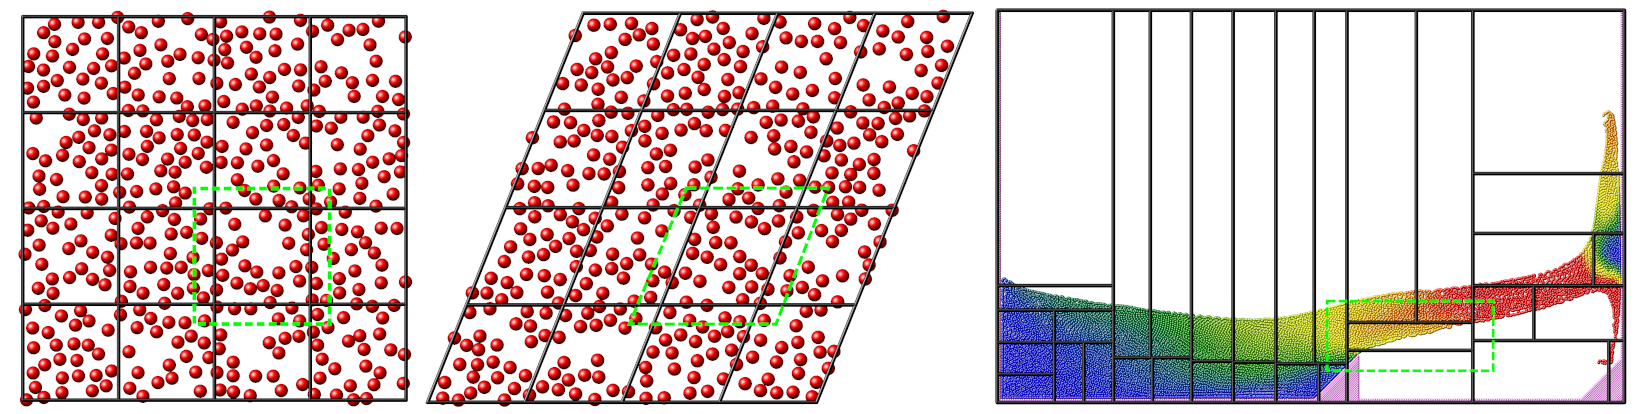
\includegraphics[width=0.9\textwidth]{domain-decomp.png}

  While applications may redistribute the data to give a more standard
  distribution, it's a wasted step - we can just consume the data directly.

  \medskip

  The API would take the per-rank domain size and index offset.
  
\end{frame}

\begin{frame}
  \frametitle{Multi-GPU: Targets of Opportunity}

  We've had an ask for multiple (ie 2) batch dimensions.  We can
  extend this API in the multi-gpu (single/multi node) header without
  modifying \texttt{rocfft.h}.  

  \bigskip
  
  Spectral ops can be greatly optimised in a multi-gpu setting.
  Including spectral ops in rocFFT will enable us to do this.  (This
  is unscoped even for single-GPU.)

\end{frame}


\end{document}
